\documentclass[10pt]{article}

% Allow Unicode input (alternatively, you can use XeLaTeX or LuaLaTeX)
\usepackage[utf8]{inputenc}
\usepackage{amssymb,amsmath,latexsym,amsfonts,amsthm,mathtools}
\usepackage{hyperref}

\usepackage[left=0.75in,right=0.75in,top=1in,bottom=1in]{geometry}
\usepackage{float}
\usepackage[justification=centering,font=footnotesize,skip=0pt]{caption}

\usepackage{microtype,xparse,tcolorbox}
\newenvironment{reviewer-comment }{}{}
\tcbuselibrary{skins}
\tcolorboxenvironment{reviewer-comment }{empty,
  left = 1em, top = 1ex, bottom = 1ex,
  borderline west = {2pt} {0pt} {black!20},
}
\ExplSyntaxOn
\NewDocumentEnvironment {response} { +m O{black!20} } {
  \IfValueT {#1} {
    \begin{reviewer-comment~}
      \setlength\parindent{2em}
      \noindent
      \ttfamily #1
    \end{reviewer-comment~}
  }
  \par\noindent\ignorespaces
} { \bigskip\par }

\NewDocumentCommand \Reviewer { m } {
  \section*{Comments~by~Expert~Reviewer~#1}
}

\ExplSyntaxOff
\AtBeginDocument{\maketitle\thispagestyle{empty}\noindent}

% You can get probably get rid of these definitions:
\newcommand\meta[1]{$\langle\hbox{#1}\rangle$}
\newcommand\PaperTitle[1]{``\textit{#1}''}

\title{Statement on the revision of \textsc{CYB-E-2018-01-0122} based on the referees' report}
\author{Abhinav Sinha \and Rishemjit Kaur \and Ritesh Kumar \and Amol P. Bhondekar}
\date{\today}

\begin{document}
We would like to express our deepest gratitude to the editor and the expert reviewers for their valuable suggestions that have helped us in improving the quality of our manuscript.\medskip

\noindent This statement concerns our revision of the manuscript \emph{CYB-E-2018-01-0122} entitled \PaperTitle{Consensus based odour source localisation by multi-agent systems} submitted to the IEEE Transactions on Cybernetics, based on the referees' report. We have made the required changes suggested by the expert reviewers in the revised manuscript and have addressed their concerns in this document.

\section*{Comments by the Associate Editor}
\begin{response}{Three valid review reports have been returned. All the reviewers find that the paper deserves a publication, but is subject to necessarily significant revisions from both technical and writing aspects, particularly for the concerns raised by Reviewer 2. Moreover, some writing typos should be corrected, which has been pointed out by all the reviewers. Based on the reviewers’ comments and handling AE’s assessment, the paper is acceptable for publication after making the changes as suggested by the reviewers.}

With your kind suggestion, we have tried to address the concerns of expert reviewers and improve the quality of the manuscript.

\end{response}


\Reviewer{\#1}
This paper studied odour source localisation of heterogeneous multi-agent systems. Nonlinear and heterogeneous agent dynamics have been addressed using sliding mode control, which improves the state of the art. In a nutshell, the contributions of this paper are solid. Therefore, I recommend acceptance of this paper after carefully addressing the following concerns

\begin{response}{Some remarks about the conservativeness of the assumptions in this work should be provided}

Odour source localisation is a challenging problem from many fronts. As of now, we have limited our scope to the cooperative control aspects only. Every approach has its pros and cons, and to build something we need to make certain assumptions. Here, we briefly discuss the conservativeness of the assumptions, which we have also included in the revised manuscript.

If the domain of localisation is very large, the number of agents should increase in order to effectively solve OSL problem. However, increase in number of agents shall add to the economy, and there is a cost to maintain the communication links. Further, anomalies such as packet dropout, link failure and latencies in communication should be carefully checked. Another scenario where localisation is quite difficult, if not impossible, is the presence of multiple time varying global maxima and local minima. This shall render MAS slightly confused and a different approach should be adopted, such as extrapolating the location based on known (or probable) presence of the source.
\end{response}

\begin{response}{Where does the forcing function (26) come from? Please clarify it.}

Sliding mode control is characterised by two phases-- the reaching phase and the sliding phase. In the reaching phase, state trajectories emanate from various locations in state space and move towards the sliding hyperplane. During this segment of time, tracking error can't be controller directly and hence, the response of the system can be adversely affected by parameter variations and noise. Thus, it would be pragmatic to reduce this period (or even eliminate it). A simplest way to shorten the reaching time is to incorporate a control with higher magnitude of gain. This, in turn, might excite unmodelled plant dynamics and can cause wear and tear of the hardware. This near infinite frequency switching is called chattering, and is an undesirable phenomenon. While electronic switching systems may exploit this phenomenon to their advantage, mechanical hardware in mechatronic systems may degrade, eventually leading to failure. 

Traditional reaching laws in the literature of sliding mode employ a control effort of fixed gain. In order to shorten the reaching time, a larger control input was designed, leading to chattering. On the contrary, we have designed the gain to be nonlinear by using an inverse sine hyperbolic function. This function is odd and monotonous. Whenever the trajectories are away from the surface, the gain is high and they are pulled towards the hyperplane quickly, and when the trajectories are near the hyperplane, the gain is reduced to avoid chattering. This variable gain in the reaching law results in a smoother control signal as opposed to a discontinuous one.

Traditional reaching law is given by
\begin{equation}\label{sdotold}
\dot{s}_i(t) = -\mu \; sign(s_i(t)),
\end{equation}
where $\mu$ is the fixed gain. The forcing function (sliding mode reaching law) in our discussion is
\begin{equation}\label{sdot}
\dot{s}_i(t) = -\mu \sinh^{-1}(m + w|s_i(t)|) sign(s_i(t)),
\end{equation}
in which $\mu \sinh^{-1}(m + w|s_i(t)|)$ is the variable gain. A similar reaching law has been used in \cite{6512130,Sinha2016,Majumder2018155}.
\begin{figure}[h!]
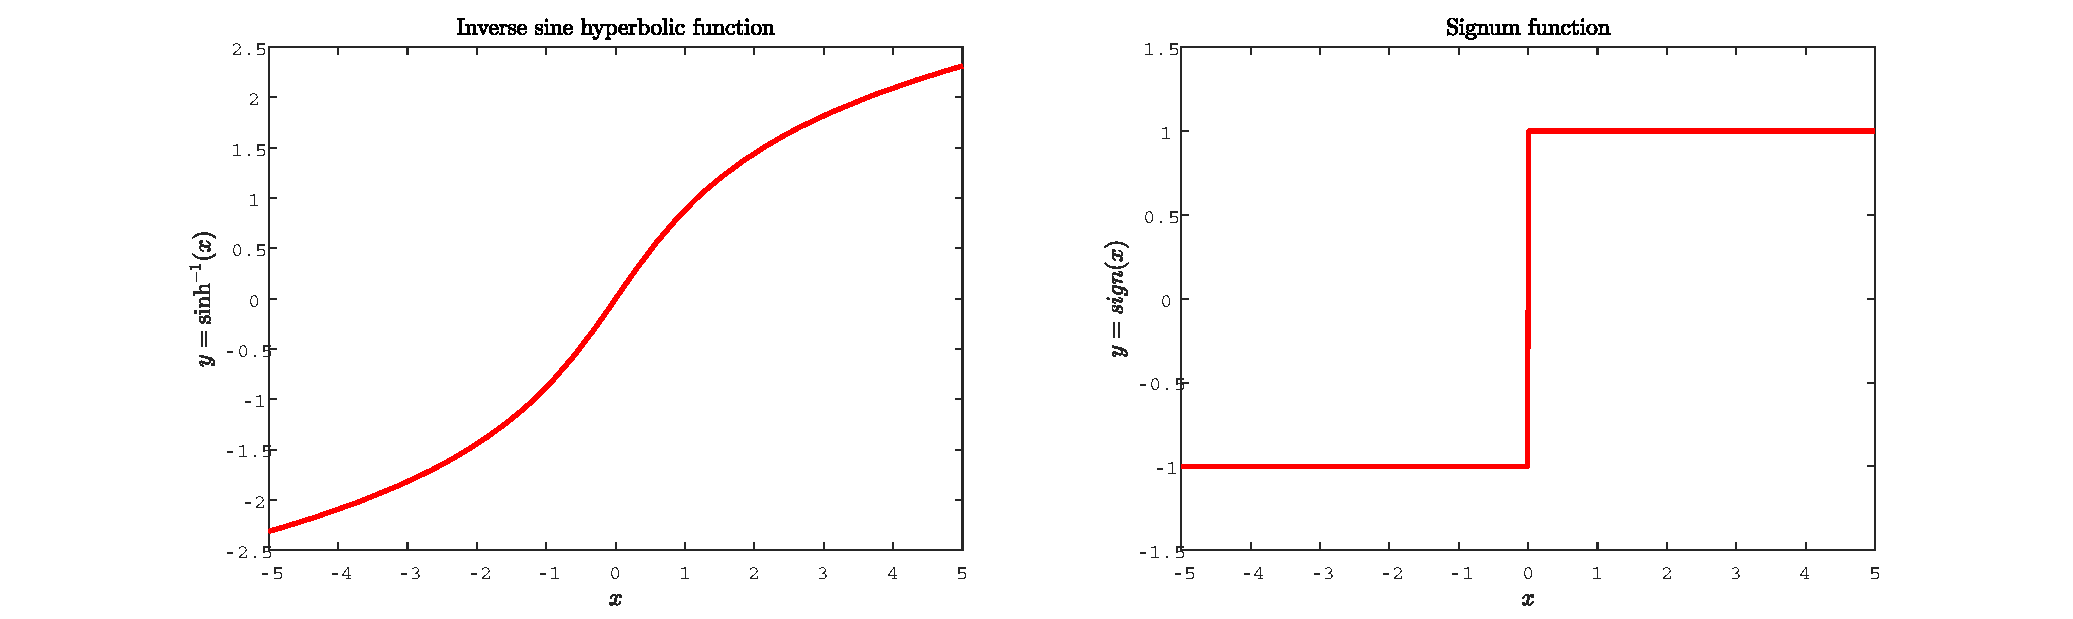
\includegraphics[width=\textwidth]{sinhandsign.pdf}\caption{Inverse sine hyperbolic and signum functions}
\end{figure}


Note that the $\sinh^{-1}(\cdot)$ is smooth and increases (decreases) with increase (decrease) in the argument.
\end{response}

\begin{response}{Figures 8 and 9 are not very clear.}
Figures 8 and 9 depict the velocity plots of the turbulence in the domain of localisation. Due to page limitations in the main manuscript, we have moved figures 8 and 9 to a supplementary file. The domain of localisation is characterised by heavy turbulence. Hence, we have taken snapshots in different segments of time to illustrate the turbulence using velocity plots. In both the figures, there are four snapshots. The first snapshot is taken randomly between $t = 0$ and $t = 2.5$ sec. Similarly other snapshots are taken between $t = 2.5$ and $t = 5$ sec, $t = 5$ and $t = 7.5$ sec, and $t = 7.5$ and $t = 10$ sec. Length of the arrow corresponds to the magnitude of the wind velocity and the direction of the arrow signifies the direction of wind flow.

\end{response}

\begin{response}{Fix some typos.}
We express our sincere apologies. As per your kind suggestion, we have tried to rectify the typographical errors in our revision.

\end{response}

\Reviewer{\#2}
This paper presents an investigation of the task of localising unknown source of an odour in the framework of heterogeneous multi-agent systems. A hierarchical cooperative control strategy has been proposed as a potential candidate to solve the problem. Some comments are listed as follows.

\begin{response}{In section "A Group Decision Making”, the proposed algorithms seems complicated and confused.}

Group decision making layer utilises standard PSO to kick-start the search process. In this scheme, each agent is regarded as a particle. Each agent adjusts its state according to its own experience and that of its neighbours by tracking two positions-- the best position so far found out by the agent itself (referred as the local best), and the best position found out by its neighbours (referred as the global best).

Each agent can sense the concentration of odour molecules via sensors equipped on it. Thus, concentration information can be easily obtained. Although a probable location of the odour source can be found out using this concentration information alone, it is not so accurate because the effect of wind is decisive in shaping the odour plume. Hence, it is pragmatic to include the wind information to make a more accurate prediction. That is why the probable location in our study is given as the weighted (and balanced) sum of concentration information and wind information (equation $6$). Now this location becomes the target to be tracked for which the control algorithm is used.

To summarise, concentration information is obtained via swarm algorithm, and the wind information is obtained using a measurement model that describes the movement of odour molecules. Combining these two information together gives the probable location of the odour source, which is fed to the tracking controller.

\end{response}

\begin{response}{In section "C Distributed Control”, the control algorithms are decentralized, but not distributed. Besides, the algorithm does not depend on the topology.}

Each agent executes its own control algorithm individually. Every autonomous agent is equipped with small embedded systems as control stations. The control stations are distributed throughout the domain as the agents search the area, hence we have used the term distributed even if there is no central controller.

As per the suggestion of the expert reviewer, we have rectified the same to decentralised control in our revision. There is communication between controllers, though not explicitly shown mathematically. For our future work, we have started working on resource efficient distributed and decentralised control for odour source localisation.

\end{response}

\begin{response}{In Fig 3, it seems from the trajectories that some agents have cross the source before consensus convergence. Some explanations should be added to state the case.}

Fig 3 in the main manuscript presents a particular case of localisation in $\mathbb{R}^1$. The odour source is randomly placed between $10$ m and $11$ m, as shown in figure \ref{fig:xi}. This means that there is a global concentration maximum between $10$ m and $11$ m. Agents and their respective trajectories are represented by five different colours. The odour source is represented by a grey circle, and the filaments released from the odour source are represented as black dots. Agents start from various initial conditions that are far from the origin. Agents start moving from left hand side to progress towards the source via instantaneous plume sensing (by sensing odour molecules, or filaments). As soon as the leader agent senses the odour molecules, the information of predicted next state is exchanged among other agents. This local information is then used to make a consensus while localisation. It is worthy to note that agents do not cross the source prior to the establishment of consensus. It is also evident that agents come to consensus in finite time to locate the odour source.
\begin{figure}[h!]
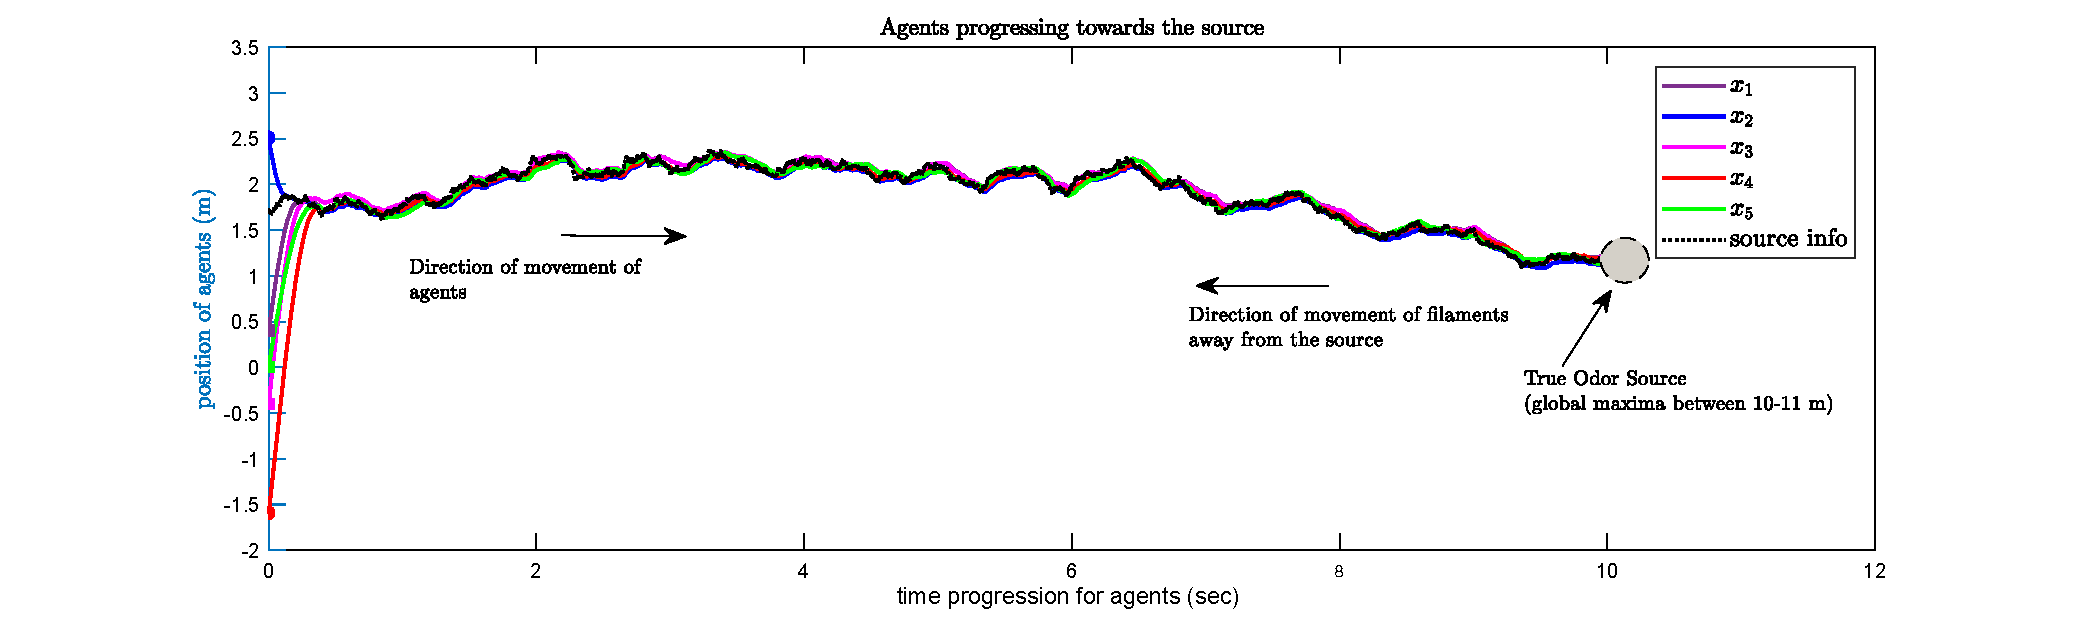
\includegraphics[width=\textwidth]{xiR1.pdf}
\caption{Consensus based localisation in $\mathbb{R}^1$.}\label{fig:xi}
\end{figure}

Kindly note that due to page limitations in the main manuscript, we have moved figure3 to a supplementary file.
\end{response}

\begin{response}{This paper just consider the stationary source, which is a very simple problem. A general dynamical source model should be adopted to show the effectiveness of proposed hierarchical strategy.}

Type your response here.

\end{response}

\begin{response}{Grammar and equations should be checked carefully.}
Grammar and equations have been checked thoroughly in the revision.

\end{response}

\Reviewer{\#3}
his paper presents an interesting hierarchical distributed cooperative scheme, employed within the framework or odor source localization, to achieve group decision making and consensus convergence. Beyond the use case itself, this is the most interesting (and detailed) part of the contribution.

\begin{response}{There are many little improvements that are necessary leading to a substantial revision. First of all language could be check and also the grammar: pay attention to little things like punctuation and spaces.}

Our sincere apologies for the little mistakes in grammar and punctuations. In the revision, we have tried to rectify the silly mistakes.

\end{response}

\begin{response}{As second, the quality of figures sometime is very low (fig. 1 seems not being vectorial image format). Then also the final plots needs revision: the idea is good but the presentation is horrible. Titles and legends have different fonts and sizes and they shall ideally done with the same tool, using same style. Also about content, just to make an example: what's the info provided by 10 sec snapshot for Fig 5? It would have been the same cutting it out at 2 second, right? Same observation for other plots: please cut unnecessary parts and make lines more visible and central.}

As per your suggestion, we have incorporated the changes and tried to improve the quality of figures.

\end{response}

\begin{response}{Last but not least, the assumptions in that form within the Results section are not properly placed. I would have put them rather in the model description, not in the discussion phase.}

We have moved the assumptions provided in the discussions section to the model description section.

\end{response}

\bibliographystyle{IEEETran}
\bibliography{references}


\end{document}